\documentclass[9pt,a4]{article}

\usepackage[utf8]{inputenc}
\usepackage[T1]{fontenc}

\usepackage[margin=0.5cm,landscape,twocolumn]{geometry}
\setlength{\columnsep}{1cm}
\setlength{\columnseprule}{0.1pt}

\newcommand{\noun}[1]{\textsc{#1}}

\usepackage[strict]{changepage}

\usepackage{tikz}
\usepackage{background}
\usepackage[hyphens]{url}

%\usepackage{pdflscape}
%\usepackage{multicol}

\begin{document}

\pagenumbering{gobble}

\backgroundsetup{%
    scale=1.45,hshift=0cm,vshift=1cm,angle=0,contents={%
        \begin{tikzpicture}
            %\pgfmathsetmacro{\myopacity}{mod(\thepage-1,4)*0.25+0.25}
            \node[opacity=0.25] {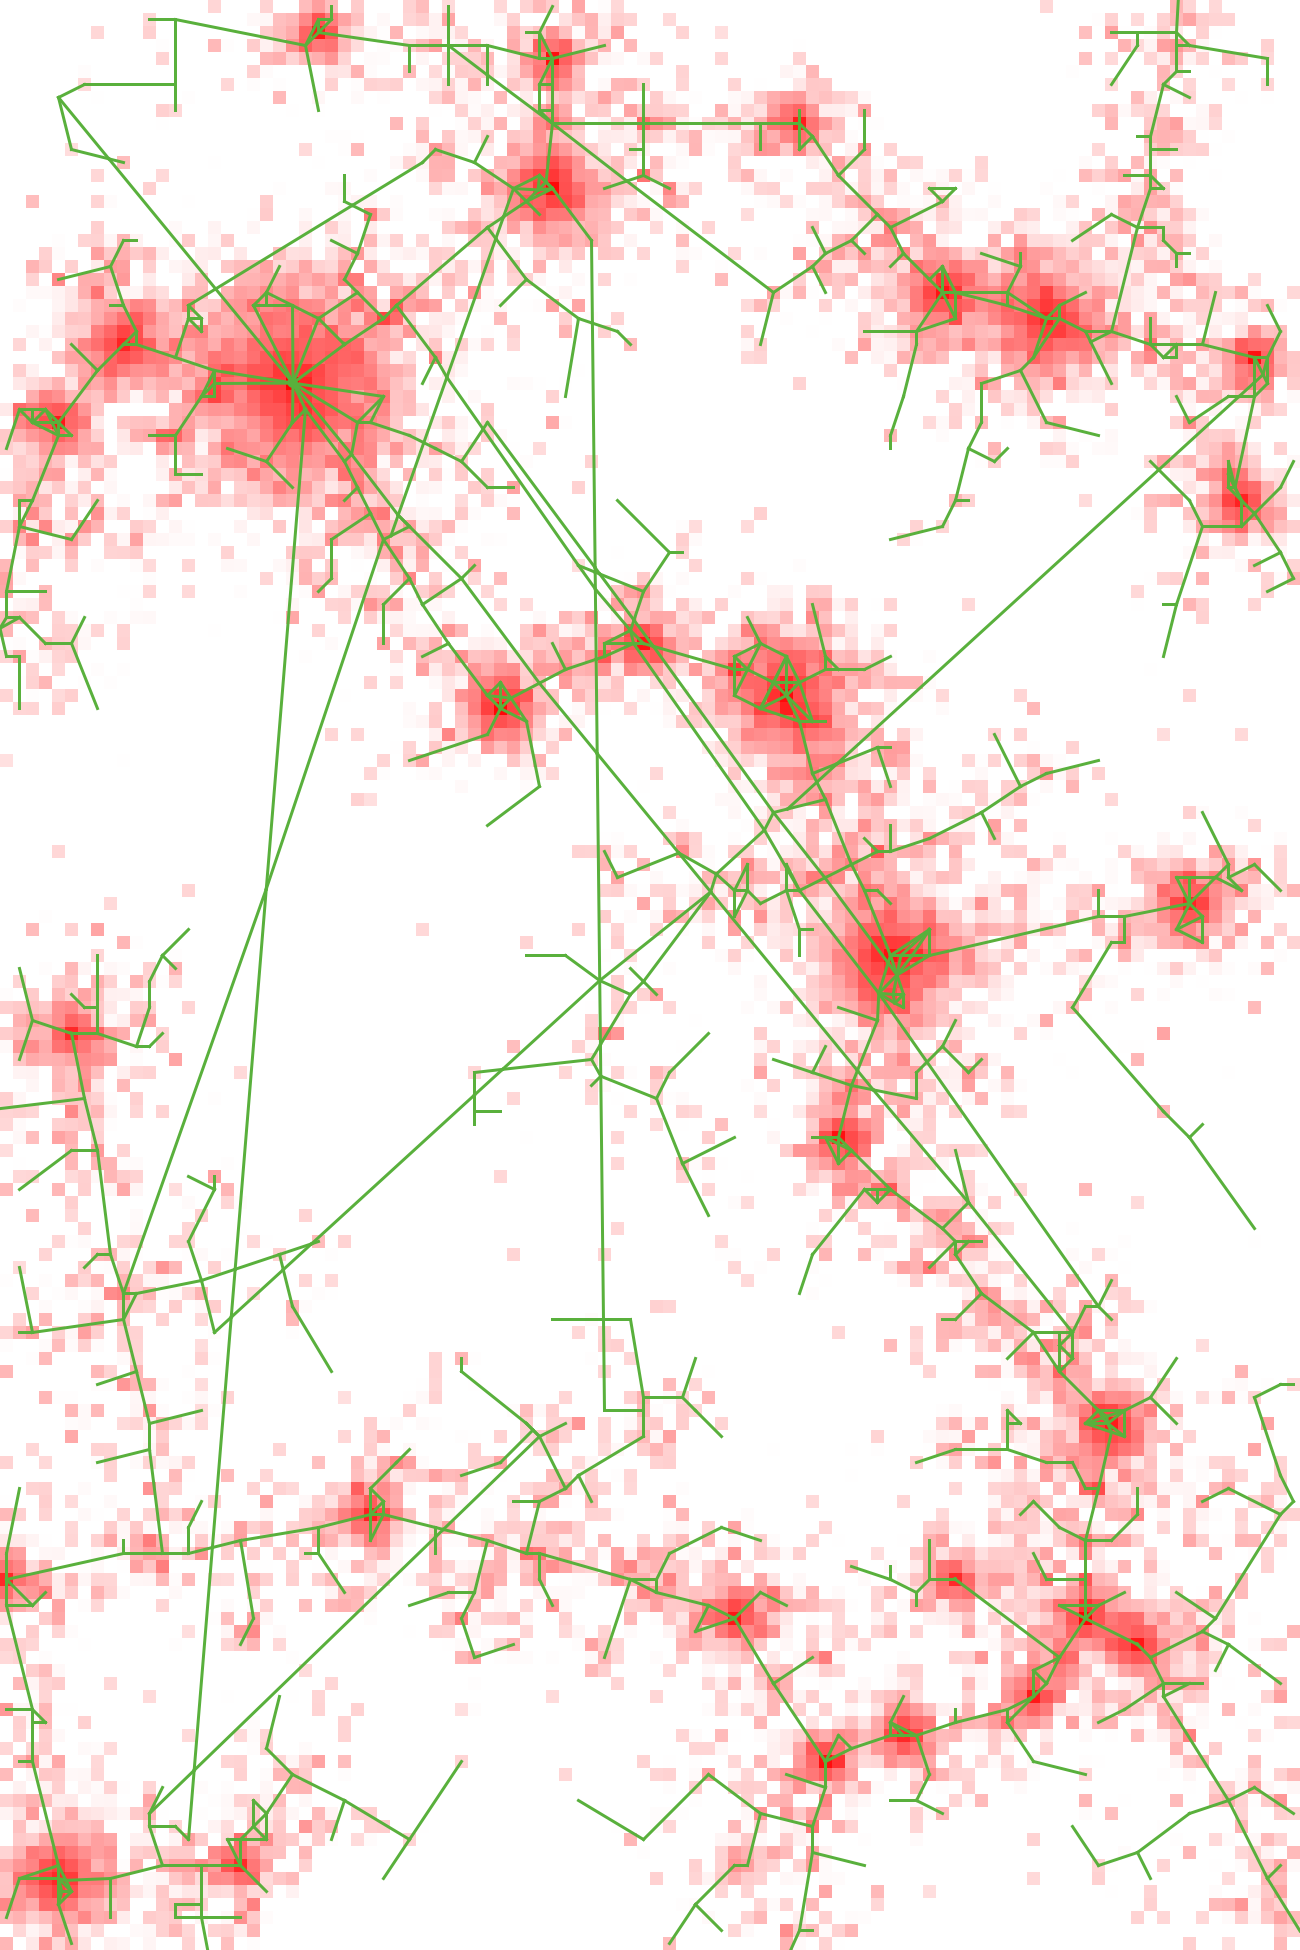
\includegraphics[width=1.35\linewidth,angle=90]{../Figures/Cover/cover2}};
        \end{tikzpicture}
    }
}



%\begin{landscape}



\null
\vspace{1cm}

{
\center
\huge

\textbf{Soutenance de Thèse et Séminaire}

\vspace{1cm}

\Large

\textit{Lundi 11 juin 2018}

\medskip


\textit{Institut des Systèmes Complexes\\
113 rue Nationale, 75013 Paris
}



}


\vspace{1cm}


\section*{Programme}

\subsection*{Séminaire}

\textit{De 9h30 à 11h30, séminaire interdisciplinaire autour des épistémologies et pratiques de la modélisation urbaine, avec présentations de : }

\medskip

\noindent\textbf{Denise Pumain} (Université Paris 1), \textbf{Alain Bonnafous} (Université Lumière Lyon 2), \textbf{Clémentine Cottineau} (CNRS), \textbf{Vincent Viguié} (CIRED).

\vspace{0.5cm}


\subsection*{Soutenance de Thèse}

\textit{A 14h, soutenance de Thèse en Géographie à l'Université Paris Diderot par }

\medskip

\noindent\textbf{Juste Raimbault} (UMR CNRS 8504 Géographie-cités, UMR-T 9403 IFSTTAR LVMT)

\medskip

\noindent\textit{présentée devant le jury composé de}

\medskip

\noindent
\begin{minipage}{0.32\linewidth}
\raggedright
\textbf{\noun{Denise Pumain}}\\
\textbf{\noun{Didier Josselin}}\\
\textbf{\noun{Catherine Morency}}\\
\textbf{\noun{Olivier Bonin}}\\
\textbf{\noun{Anne Ruas}}\\
\textbf{\noun{Arnaud Banos}}\\
\textbf{\noun{Florent Le Néchet}}
\end{minipage}
\begin{minipage}{0.75\linewidth}
\raggedright
Professeure, Université Paris 1, Présidente du Jury\\
Directeur de Recherche, CNRS, Rapporteur\\
Professeure, Ecole Polytechnique de Montréal, Rapporteuse\\
Chargé de Recherche, IFSTTAR, Examinateur\\
Directrice de Recherche, IFSTTAR, Examinatrice\\
Directeur de Recherche, CNRS, Directeur\\
Maître de Conférences, Université Paris-Est, Directeur\\
\end{minipage}

\bigskip
\bigskip

\noindent\textit{Merci de confirmer votre présence à la soutenance et/ou au séminaire par email à }\texttt{juste.raimbault@iscpif.fr}

\newpage

\null
\vfill

\section*{Résumé de la thèse}
%Short summary of the contents\dots a great guide by 
%Kent Beck how to write good abstracts can be found here:  
%\begin{center}
%\url{https://plg.uwaterloo.ca/~migod/research/beckOOPSLA.html}
%\end{center}

\textbf{Caractérisation et modélisation de la co-évolution des réseaux de transport et des territoires}

\bigskip

\noindent\textbf{Mots-clés : } Territoires ; Réseaux de Transport ; Co-évolution ; Morphogenèse ; Théorie Évolutive des Villes ; Épistémologie Quantitative ; Systèmes de Villes ; Morphologie Urbaine ; Grand Paris ; Delta de la Rivière des Perles

\bigskip

\noindent
L'identification d'effets structurants des infrastructures de transports sur la dynamique des territoires reste un défi scientifique ouvert. Cette question est une des facettes de recherches sur la complexité des dynamiques territoriales, au sein desquelles territoires et réseaux de transport seraient en co-évolution. L'objectif de cette thèse est de mettre à l'épreuve cette vision des interactions entre réseaux et territoires, autant sur le plan conceptuel que sur le plan empirique, en les intégrant au sein de modèles de simulation des systèmes territoriaux. La nature intrinsèquement pluri-disciplinaire de la question nous conduit à mener un travail d'épistémologie quantitative, qui permet de dresser une carte du paysage scientifique et une description des éléments communs et des spécificités des modèles traitant la co-évolution entre réseaux et territoires dans chaque discipline. Nous proposons ensuite une définition de la co-évolution, ainsi qu'une méthode de caractérisation empirique, basée sur une analyse de corrélations spatio-temporelles. Deux pistes complémentaires de modélisation, correspondant à des ontologies et des échelles différentes sont alors explorées. A l'échelle macroscopique, nous construisons une famille de modèles dans la lignée des modèles d'interaction au sein des systèmes de villes développés par la Théorie Evolutive des Villes (Pumain, 1997). Leur exploration montre qu'ils capturent effectivement des dynamiques de co-évolution, et leur calibration sur des données démographiques pour le système de villes français (1830-1999) quantifie l'évolution des processus d'interaction comme l'effet tunnel ou le rôle de la centralité. A l'échelle mésoscopique, un modèle de morphogenèse capture la co-évolution de la forme urbaine et de la topologie du réseau. Il est calibré sur les indicateurs correspondants pour la forme et la topologie locales calculés pour l'ensemble de l'Europe. De multiples processus d'évolution du réseau s'avèrent être complémentaires pour reproduire la grande variété des configurations observées, au niveau des indicateurs ainsi que des interactions entre indicateurs. Ces résultats suggèrent de nouvelles pistes d'exploration des modèles urbains intégrant les dynamiques co-évolutives dans une perspective multi-échelles.

\bigskip

\noindent\textit{Mémoire de thèse disponible à }\\\raggedright\url{https://github.com/JusteRaimbault/ThesisMemoire/raw/master/Final/Versions/Raimbault_Memoire_v3.5.3.pdf}

\bigskip

\noindent\textit{Dépôt git à }\url{https://github.com/JusteRaimbault/CityNetwork}

\vfill
\null

%\end{landscape}

\end{document}

